\documentclass{llncs}

\usepackage{makeidx}  
\usepackage{amsmath}
\usepackage{amsfonts}
\usepackage{amssymb}
\usepackage{listings}
\usepackage{graphicx}
\usepackage[rightcaption]{sidecap}

\usepackage{hyperref}

\begin{document}

         % for the preliminaries
%
\begin{abstract}
    \dots
    En este paper se aborda sobre la recuperaci\'on de im\'agenes, una de las ramas de la
    recuperaci\'on de informaci\'on, sus principales m\'etodos como el basado en keywords
    (keyword based image retrieval) o el basado en contenido (content based image retrieval),
    entre otros. Las ventajas y desventajas de estos m\'etodos y que aplicaciones reales tiene 
    la recuperaci\'on de im\'agenes .

   \keywords{content-based image retrieval, keyword-based image retrieval, image retrieval,}
\end{abstract}

\tableofcontents
%

  
          % start of the contributions

%
\title{Caracter\'isticas del problema}
%
\titlerunning{}  % abbreviated title (for running head)
%                                     also used for the TOC unless
%                                     \toctitle is used
%



%
\author{David Orlando De Quesada Oliva, Javier Dom\'inguez}
%
\authorrunning{Ivar Ekeland et al.} % abbreviated author list (for running head)
%
%%%% list of authors for the TOC (use if author list has to be modified)

%
\institute{MATCOM, Universidad de La Habana,\\
\email{d.quesada2@estudiantes.matcom.uh.cu, j.dominguez@estudiantes.matcom.uh.cu},\\
\texttt{}
}

\maketitle



La Recuperación de im\'agenes es el campo que se encarga de buscar y obtener imágenes 
digitales de una base  de datos. Debido a la cantidad creciente de imágenes digitales 
alrededor del mundo, desde 1970 este campo ha estado bien activo. Un sistema de 
recuperación efectivo y rápido de imágenes necesita operar sobre una colección de 
imágenes y devolver las imágenes relevantes basadas en la consulta, la cual 
se realiza lo más cercana posible a la percepción humana. Los investigadores de este 
campo poco a poco, han ido mejorando e implementando varios tipos de sistemas de recuperación 
de imágenes, de los sistemas basados en \textbf{palabras claves}, pasando por los sistemas 
basados en el contenido (características) de una imagen, y finalmente llegando a los 
sistemas de recuperación semánticos, con el objetivo de reducir el vacío semántico que 
existe entre la representación de características de bajo nivel (color, textura, forma, etc) y 
la semántica de alto nivel en las imágenes.

Desarrollar un motor de búsqueda de imágenes omnipotente, capaz de satisfacer a todos los usuarios 
requiere entender y caracterizar la interacción y la búsqueda de imágenes desde el punto de vista 
del usuario y del sistema. Desde el punto de vista del usuario, claridad en lo que desea, donde lo 
quiere buscar y de que forma quiere realizar su consulta. Desde el punto de viste del motor de 
búsqueda, como desea el usuario que le sean presentados los resultados de su consulta, dónde desea 
buscar el usuario y cual es la naturaleza de la consulta del usuario.


\newpage
\title{Diferencias entre Image Retrieval y Content-based image retrieval}
\author{David Orlando De Quesada Oliva, Javier Dom\'inguez}
\institute{MATCOM, Universidad de La Habana,\\
\email{d.quesada2@estudiantes.matcom.uh.cu, j.dominguez@estudiantes.matcom.uh.cu},\\
\texttt{}
}
\maketitle


La recuperación de imágenes (Image Retrieval) se refiere a la rama de la recuperación de información que se encarga 
de dada una consulta que puede realizar un usuario de disímiles formas, devolver un ranking de las imágenes que más 
se asemejen a la consulta hecha por el usuario, teniendo en cuenta alguna medida de similitud. La recuperación de 
imágenes basada en contenido(Content-based image retrieval) se refiere a un tipo específico de método de recuperación de 
imágenes que se  caracteriza por usar el contenido de las imágenes (color, forma, textura, etc) para realizar el proceso 
de consulta.

\newpage
\title{Principales m\'etodos para la recuperaci\'on de im\'agenes}
\author{David Orlando De Quesada Oliva, Javier Dom\'inguez}
\institute{MATCOM, Universidad de La Habana,\\
\email{d.quesada2@estudiantes.matcom.uh.cu, j.dominguez@estudiantes.matcom.uh.cu},\\
\texttt{}
}
\maketitle

\section*{Keyword Based Image retrieval:}

En un \textbf{image retrieval system convencional}, los \textbf{keywords} son 
usados como descriptores para indexar y recuperar una imagen.  Las palabras 
claves (key words) no transmiten mejor que el contenido de una imagen 
el significado de esta. Antes de que las imágenes sean almacenadas en la base de datos, son examinadas 
manualmente y se les asigna una palabra  clave (\textbf{keyword}) para describir su 
contenido. Estos  keywords  son almacenados como parte de los atributos 
asociados a la imagen. En el proceso de hacer una consulta, el sistema 
aceptará del usuario una o varias \textbf{keywords} que serán el criterio de búsqueda.
Luego se realiza un proceso para encontrar las imágenes que cumplen con el criterio 
de búsqueda. Las t\'ecnicas de text based image retrieval usan texto para describir el 
contenido de una imagen lo que a menudo crea ambig$\ddot{u}$edad e insuficiencia en el 
procesamiento de la query y el rendimiento en una b\'usqueda de la base de datos de 
im\'agenes. El proceso de asignaci\'on de meta datos con captions o keywords a una imagen
digital es conocido como anotaci\'on autom\'atica de im\'agenes(automatic image anotation).
Este tipo de text based informacion retrieval est\'a motivado l\'exicamente en lugar de 
conceptualmente, lo que lleva a resultados de b\'usqueda irrelevantes en la recuperaci\'on en la 
recuperaci\'on de informaci\'on.
\\
\begin{SCfigure}[0.5]
    \caption{Proceso general de un keyword based image retrieval}
    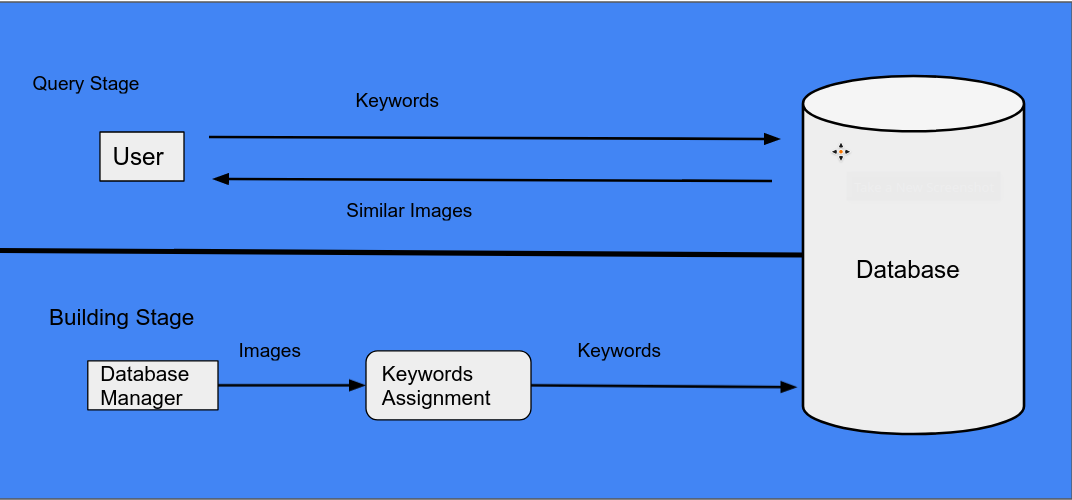
\includegraphics[scale = .3]{./images/kbir-process.png}
\end{SCfigure}





\subsection{Text Based Image Retrieval:}

Las t\'ecnicas b\'asicas de recuperaci\'on de documentos pueden ser usadas para la recuperaci\'on
de im\'agenes basadas en metadatos sin modificaci\'on. En un keyword based image
retrieval, los metadatos que describen las im\'agenes pueden ser categorizados en 2
partes. Una parte se refiere a las herramientas usadas en el proceso de creaci\'on de la imagen, estilo de
de arte de la imagen, artista, precio, y otras propiedades expl\'icitas de la imagen. La otra parte describe
lo que realmente hay en la imagen, las propiedades imp\'icitas que pueden entenderse al 
percibir la imagen en si. En el contexto actual de la recuperaci\'on, el texto plano anotado en im\'agenes
responde de manera similar al texto plano en documentos, debido a que ambos contienen texto, lo cual permite
que sean explotados por las t\'ecnicas convencionales de text-bases information retrieval. La recuperaci\'on de
informaci\'on basada en texto gen\'erica se realiza de tal manera que inicialmente el usuario reliza una
consulta(query) que tiene de 1 a m \textbf{keywords}. En los sistemas de recuperaci\'on basados en 
metadatos(metadata based information retrieval), el buscador compara los keywords con un conjunto de im\'agenes 
recopiladas de una base de datos y les da prioriad a los valores. Por ejemplo, si el keyword es \textbf{book}, y la 
imagen A contiene 2 ocurrencias de book y la imagen B solo una ocurrencia, entonces A tiene una prioridad mayor.  Las 
im\'agenes con palabras claves anotadas son mostradas al usuarios en el orden de reducci\'on de la prioridad. Im\'agenes 
irrelevantes son recuperadas y el usuario tiene que gastar tiempo en el filtrado de la informaci\'on, usualmente navegando
a trav\'es de los resultados de b\'usqueda. 

\subsection{Field Based Image Retrieval:}
Field based retrieval es una extensi\'on del text based retrieval donde solo un campo(field) es usado en anotaci\'on 
y recuperaci\'on. El enfoque basado en el campo (field based) describe y recupera art\'iculos usando uno o m\'as pares de valores 
del campo. Regularmente un esquema de metadatos es descrito por un conjunto de campos y pocas indicaciones sobre el tipo de
valores que puede ser elegidos por un campo  particular. La plantilla (template) de metadatos y esquemas ampliamaneta utilizada para 
describir documentos online en general es la \textbf{Dublin Core(DC)}. Los campos de la DC version 1.1 son rights, coverage, relation,
language, source, identifier, format, type, data, contributor, publisher, description, subject, creator y title.  Versiones calificadas de 
DC han sido creadas para dominions particulares como la decripci\'on de piezas de arte en museos.

\subsection{Structure Based Image Retrieval:}

El paradigma de recuperaci\'on basado en estructuras. En este m\'etodo, se utiliza un enfoque basado enn el campo(field) que principalmente
utiliza una estructura de parers de valores atributo. Este m\'etodo permite descripciones m\'as complejas implicando relaciones. Por ejemplo,
una definici\'on de una parte de un auto puede incluir especificaciones de esos componentes. Cada elemento del objeto se puede especificar 
de nuevo usando varios atributos como la forma, el tama\~{n}o y el material. Los elementos pueden incluso tener elementos ellos mismos, por 
ejemplo, una mesa tiene patas, y sus subelementos pueden moverse hasta el nivel donde un elemento no puede obtener un subelemento m\'as particular.

\section{Content Based Image Retrieval(CBIR):}

El Content Based Image Retrieval(CBIR) es uno de los m\'etodos de visi\'on por computadoras para la recuperaci\'on de
im\'agenes, lo que significa que para poder recuperar es necesario im\'agenes digitales de una base de datos de im\'agenes. 
La b\'usqueda basada en contenido(Content based search) realizar\'a el an\'alisis con el contenido real de la imagen, en 
lugar de metadatos como etiquetas(tags), palabras clave(keywords), o descripciones anotadas con la imagen. La palabra 
contenido aqu\'i puede referirse a formas, color, texturas o alg\'un otro detalle que se puede obtener dentro de la propia
imagen. El motor de búsqueda de imágenes relacionadas con la web se basa en metadatos, por lo que genera una gran cantidad 
de resultados basura. Por lo tanto CBIR es deseable en este caso. D\'andole palabras clave (keywords) de forma manual a las 
im\'agenes de b\'usqueda en una larga base de datos puede obtener resultados incorrectos. Adem\'as el proceso es costoso y 
puede que no identifique todas las palabras clave(keywords) que especifican la imagen y, por tanto, es ineficiente. Al 
proporcionar una buena técnica de indexación basada en el contenido real de las imágenes, se puede recuperar y producir
resultados precisos.

\subsection{Low-Level Image Feature:}

Para poder realizar el CBIR las caracter\'istics de bajo nivel de la imagen  (low-level image feature) deben ser extra\'idas 
primero. La extracci\'on de caracter\'isticas puede hacerse en toda la imagen o solo en una regi\'on de inter\'es. La t\'ecnica
simple usada en la recuperaci\'on de im\'agenes depende de las caracter\'isticas globales. La percepci\'on humana coincide 
estrechamente con la representaci\'on de im\'agenes a nivel de regi\'on. Para realizar la recuperaci\'on de im\'agenes 
basada en regiones el paso m\'as importante es la segmentaci\'on de im\'agenes. De la regi\'on segmentada, las caracter\'isticas 
de bajo nivel como textura, el color, la forma o la ubicaci\'on espacial se pueden extraer f\'acilmente. Basado en las caracter\'isticas
de la regi\'on, se puede encontrar f\'acilmente la coincidencia entre dos im\'agenes 

\subsection{ Image Segmentation}
El proceso autom\'atico de la realizaci\'on de la segmentaci\'on de una imagen es una tarea dif\'icil. Las t\'ecnicas acad\'emicas 
usadas en la segmentaci\'on de im\'agenes son curva de  difusi\'on de energ\'ia(curve energy diffusion), evoluci\'on(evolution) y particionamiento 
de grafos(graph paritioning). La mayor\'ia de los m\'etodos pueden ser apropiados solo para im\'agenes que tienen regiones con colores
similares, como los m\'etodos de direct clustering en el espacio de color. Tales m\'etodos pueden adaptarse para la recuperaci\'on de sistemas 
que funcionen con colores. Pero las escenas naturales contienen tanto colores como texturas. Aplicar segmentaci\'on en texturas resulta 
dif\'icil. Incluso en la segmentaci\'on basada en texturas la estimaci\'on del par\'ametro del modelo de textura es dif\'icil. Para 
superar esto el algoritmo 'JSEG' es usado. Otro algoritmo llamado segmentaci\'on Blobworld es ampliamanente utilizado. Algunos algoritmos 
de segmentaci\'on hacen uso de segmentaci\'on basada en color, en textura o en ambas. Estos algoritmos usan k-means para prop\'ositos de 
clasificaci\'on. Los bloques de una misma clase se agrupan dentro de una misma regi\'on. El algoritmo k-means con restricci\'on de 
conectividad (KMCC) es un trabajo de segmentaci\'on para segmentar objetos en las im\'agenes. Esta utilizaci\'on del algoritmo  se basa 
en la confianza en la necesidad del sistema y el uso del conjunto de datos. Es dif\'icil determinar que algoritmo proporciona mejores 
resultados. El resultado del JSEG es la textura y el color de regiones similares, pero el resultado de KMCC produce objetos que son diferentes.
El algoritmo KMCC es computacionalmente mucho m\'as exhaustivo que el JSEG. Por tanto, Blobworld y JSEG son principalmente los algoritmos usados.

\subsection { Varias caracter\'isticas de bajo nivel de las im\'agenes:}

En las diversas categor\'ias de algoritmos muy pocos se pueden aplicar en la recuperaci\'on de im\'agenes en tiempo real con 
sem\'antica de alto nivel que son:\\
$\blacksquare$  \textbf{Color:}\\
El color es la m\'as com\'un de la caracter\'isticas adoptadas en la recuperaci\'on de im\'agenes. Varios espacios de color son usados 
para definir colores . Esos espacios de color son usados en dependiendo de las diferentes aplicaciones. Los espacios de color 
m\'as usados son  RGB, LAB, LUV, HSV (HSL), YCrCb, y el hue-min-max-difference (HMMD). La covarianza del color, el histograma 
de color, y los momentos de color(color moments) son principalmente las caracter\'isticas de color usadas en RBIR(Region Based Image Retrieval).
 El color principal (leading color), el color escalable(scalable color)y el dise\~{n}o de color(color layout) son las caracter\'isticas 
de color que se utilizan principalmente en MPEG-7. Con el origen las caracter\'isticas de 3 colores, el par matiz-matiz y matiz
se construyen las invariantes de color. La sem\'antica de alto nivel no est\'a directamente relacionada con las caracter\'isticas 
de color mencionadas anteriormente. Para mapear los colores de una regi\'on a nombres de colores en sem\'antica de alto nivel,
el promedio de color de todos los pixeles  en una regi\'on podr\'ia usarse como su caracter\'istica de color. Si la segmentaci\'on
es err\'onea terminar\'a porque la regi\'on original es visualmente diferente al color promedio. Dependiendo de los resultados 
de la segmentaci\'on solo se seleccionan las caracter\'isticas de color. El color promedio no es una opci\'on deseable si la
segmentaci\'on da como resultado objetos que no tienen colores similares. En la mayor\'ia de los trabajos CBIR, las im\'agenes en color no
est\'an preprocesadas. Los filtros de color adecuados son esenciales para mejorar la eficiencia de recuperaci\'on debido a que el color 
en la im\'agenes siempre est\'a da\~{n}ado por el ruido.\\
$\blacksquare$  \textbf{Textura:}
Pocos sistemas no utilizan la textura como el color en la recuperaci\'on de im\'agenes. La textura es una caracter\'istica importante 
para describir la sem\'antica de alto nivel en la recuperaci\'on de im\'agenes porque proporciona detalles esenciales en un cat\'alogo 
de im\'agenes, ya que define el contexto de muchas im\'agenes del mundo real como nubes, ladrillos, \'arboles y telas. El resultado
de aplicar \textbf{la transformada de Wavelet}    o \textbf{el filtrado de Gabor}, medidas estad\'isticas confinadas asi como las
seis caracter\'istcas de textura de Samura, son las caracter\'isticas de textura m\'as utilizadas en el proceso de recuperaci\'on de 
im\'agenenes.  Las caracter\'istica de textura de Samura son:\\
$\blacktriangleright $ La regularidad\\
$\blacktriangleright $ Semejanza de l\'inea\\
$\blacktriangleright $ La rugosidad\\
$\blacktriangleright $ La direccionalidad\\
$\blacktriangleright $ El contraste\\
$\blacktriangleright $ La aspereza\\

De estas caracter\'isticas la aspereza, la direccionalidad y la regularidad son las m\'as importantes. Estas tres est\'an relacionadas 
con otras que son menos eficaces con respecto a la descripci\'on de la textura. Los descriptores de navegaci\'on de texturas son 
obtenidos desde \textbf{MPEG-7}. Estos son regularidad, asperza, direccionalidad. Se ha encontrado que la textura de Brodatz funcionar\'a
de manera excelente con caracter\'isticas de palabras como aleatoriedad, direccionalidad y periodicidad. Las caracter\'isticas de Tamura
no funcionan para m\'ultiples resoluciones que se consideren para la medici\'on. Las caracter\'isticas globales se ven afectadas por 
distorsiones de la imagen como diferencias de orientaci\'on debido a la distorsi\'on del punto de vista y la escala. Si las regiones
de textura en la imagen no est\'an organizadas y son similares, se producir\'ia una respuesta de recuperaci\'on deficiente para im\'agenes
de escenas naturales. El estudio de la visi\'on humana puede coincidir bastante con las caracter\'isticas de Wavelet y Gabor en la mayor 
parte de la recuperaci\'on de im\'agenes. Pero el dise\~{n}o actual del filtro de Gabor y la transformada de Wavelet solo est\'a 
destinado a im\'agenes rectangulares. Pero en un RBIR la regi\'on  de la imagen tiene formas err\'aticas. Por tanto en tal caso las 
caracter\'isticas de la textura se utilizan eficazmente. Pero para la representaci\'on de im\'agenes naturales el descriptor de histogramas
de borde (EHD) es el m\'as adecuado y eficaz.

$\blacksquare$  \textbf{Forma:}
Uno de los conceptos m\'as distintivos es la forma. Esta caracter\'istica tiene un l\'imite consecutivo de segmentos, una relaci\'on 
de aspecto, descriptores de Fourier, circularidad e invariantes de momento. El color y la textura son m\'as \'utiles en im\'agenes 
particulares de dominio , como objetos artificiales. A\'un asi las caracter\'isticas de la forma son caracter\'isticas esenciales 
pero no tienen tanta popularidad los RBIR como las caracter\'isticas de textura y color para explorar los beneficios inherentes de RBIR,
algunos sistemas podrían utilizar las características de forma como evaluadores. Por ejemplo, las características de orientación 
y excentricidad se utilizan para este propósito. La forma de una imagen puede definir la configuraci\'on de superficie  caracter\'isticas 
de un objeto, un contorno. Esto permite distinguir a un objeto de su entorno por su contorno. La representaci\'on de la forma puede 
generalmente dividirse en dos categor\'ias: basado en los l\'imites y basados en regiones. La representaci\'on de la forma basada en los 
bordes solo usa los bordes exteriores de la forma. Esto se hace describiendo la regi\'on considerada usando sus caracter\'isticas externas,
como los pixeles a lo largo del l\'imite del objeto. Pero la representaci\'on de la forma basada en la regi\'on es totalmente diferente 
al m\'etodo anterior. Utiliza la regi\'on de forma completa describiendo la regi\'on considerada sus caracter\'isticas internas; es 
decir los pixeles contenidos en esa regi\'on.
\\
$\blacksquare$  \textbf{Localizaci\'on espacial:}
No solo la textura, el color, o la forma son caracter\'isticas importantes sino tambi\'en la localizaci\'on espacial en la catalogaci\'on 
de la regi\'on. Por ejemplo una imagen que contenga \'arboles con c\'esped en el suelo podr\'ia tener caracter\'isticas de color y textura 
similares pero su localizaci\'on espacial ser diferente , normalmente las hojas de los \'arboles aparecen en la parte superior de una imagen,
mientras que las hojas que caen en la parte inferior. Las ubicaciones espaciales se definen intuitivamente como :\textbf{izquierda(left), derecha(right),
top(arriba), bottom(abajo)},seg\'un el lugar de la regi\'on en la imagen. El rect\'angulo delimitador m\'inimo (minimum bounding rectangle) y 
el centroide de la regi\'on se utilizan para encontrar la ubicaci\'on espacial.     

\section*{Semantic Based Image Retrieval:}

Ni una, ni la combinación de varias características visuales o de bajo nivel (color, textura, forma, relación espacial) pueden capturar 
completamente los conceptos de alto nivel de las imágenes. Además, debido a que el rendimiento de la recuperación de imágenes basado en 
características de bajo nivel no es satisfactorio, hay una necesidad de que la investigación vaya dirigida hacia la recuperación de 
imágenes basada en el significado semántico, tratando de utilizar el concepto cognitivo del ser humano para traducir esas 
características de bajo nivel a conceptos semánticos de alto nivel (vacío semántico). Este acercamiento permite a los usuarios 
acceder a imágenes a través de consultas por texto, la cual es más intuitiva, fácil y preferida por los usuarios para expresar 
su deseo. Como mencionamos previamente en el CBIR, las imágenes pasan por un proceso de extracción de características de bajo nivel que 
se almacena junto con las imágenes, ahora aquí, se hace necesario traducir esas características de bajo nivel a conceptos de alto nivel 
que no es capaz de comprender una máquina. Esta traducción usualmente se lleva a cabo utilizando herramientas de aprendizaje supervisado 
o no-supervisado, para asociar las características de bajo nivel con conceptos de alto nivel, los cuáles serán apuntados con palabras, 
durante el proceso de anotación de imágenes.
Como podemos ver la recuperación de imágenes basada en la semántica utiliza técnicas de los 2 mecanismos que surgieron previamente, 
la extracción de características de bajo nivel utilizada en CBIR y la anotación de imágenes utilizada en el mecanismo basado en 
palabras claves, para almacenar en la imagen palabras \textbf{keywords} que se obtengan del proceso de conversión de características de 
bajo nivel a conceptos de alto nivel propio de este nuevo mecanismo.


\section*{Ontology Based Image Retrieval:}
Ontolog\'ia significa una descripci\'on particular de una conceptualizaci\'on. Dise\~{n}a un dominio de manera formal. Con la ayuda 
de informaci\'on textual en los alrededores solo la recuperaci\'on de im\'agenes web es lograda. Hay algunos motores de recuperaci\'on 
de im\'agenes dependientes de texto todavia disponibles en la web como Yahoo y Google. Estos usan caracter\'isticas de texto como 
los nombres de archivos como \'indices para buscar im\'agenes en la web. Muchos motores de recuperaci\'on de im\'agenes est\'an todav\'ia 
bajo construcci\'on. Los descriptores de bajo nivel de estos motores est\'an lejos de las nociones sem\'anticas. El otro tipo de sistemas
solo se basa en anotaciones humanas. Por tanto, es necesario definir y hacer un enfoque intermedio para la compresi\'on de im\'agenes. 
Algunos sistemas pueden definir un dominio espec\'ifico a partir de un dominio experto  identificando vocabularios utilizados para 
para describir objetos de inter\'es. La cosa m\'as deseable en la recuperaci\'on de im\'agenes es la ontolog\'ia del concepto visual 
independiente del dominio. Este tipo de ontolog\'ia admite el reconocimiento autom\'atico basado en t\'ecnicas de procesamiento de 
im\'agenes.  En esto un dominio espec\'ifico se especifica usando una estructura de \'arbol con herarqu\'ia de clases de sus subelementos 
en cada nivel.

\begin{SCfigure}[0.5]
    \caption{Idea visual de la Ontolog\'ia}
    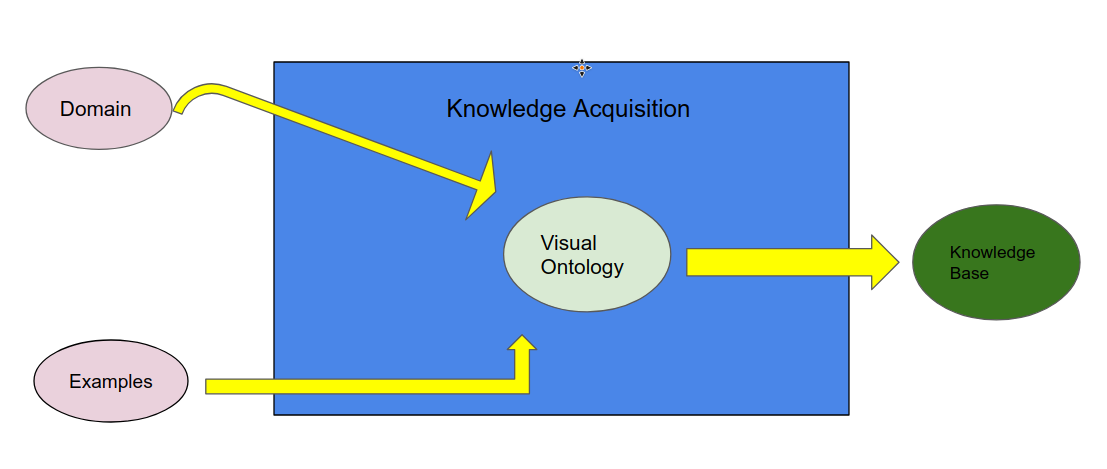
\includegraphics[scale = .3]{./images/visual_idea_ontology.png}
\end{SCfigure}

\noindent

\begin{SCfigure}[0.5]
    \caption{Arquitectura de la ontolog\'ia aplicada al proceso de recuperaci\'on de im\'agenes}
    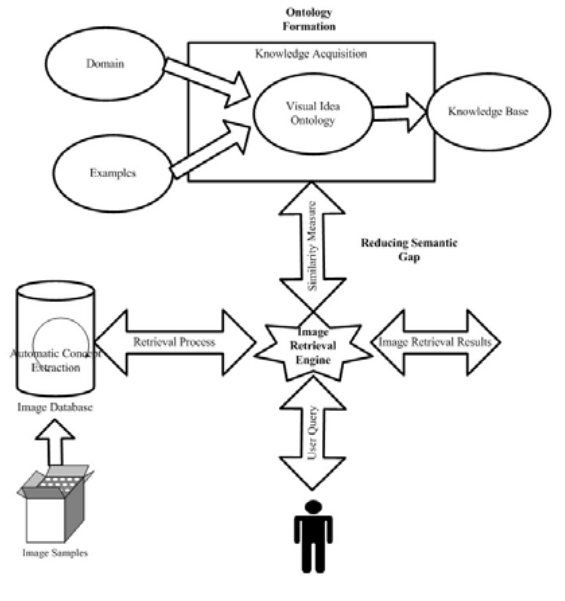
\includegraphics[scale = .4]{./images/ontolgy-bases-image-retrieval-process.png}
\end{SCfigure}

La extracci\'on de imagen hecha por una computadora puede resultar con conceptos de imagen 
significativos. Estos conceptos puede ser color, textura, forma o localizaci\'on espacial.
Mapear o m\'as de esos conceptos resultantes en ontolog\'ia interpretar\'a el significado 
conceptual de una imagen. Si la query de recuperaci\'on captura la intenci\'on actual de los
usuarios a trav\'es de la representaci\'on ontol\'ogica, definitivamente reducir\'a la disparidad 
sem\'antica entre el hombre y la m\'aquina.   

\noindent









\newpage



\title{Evaluación del sistema}
\author{David Orlando De Quesada Oliva, Javier Dom\'inguez}
\institute{MATCOM, Universidad de La Habana,\\
\email{d.quesada2@estudiantes.matcom.uh.cu, j.dominguez@estudiantes.matcom.uh.cu},\\
\texttt{}
}
\maketitle

La recuperación de imágenes es esencialmente un problema de recuperación de información. Por tanto, 
las métricas de evaluación han sido adoptados de forma bastante natural a partir de la investigación de 
recuperación de información. Dos de las Las medidas de evaluación más populares son:\\
$\blacksquare$ Precisión: el porcentaje de imágenes recuperadas que son relevantes para la consulta.\\
$\blacksquare$ Recobrado: el porcentaje de todas las imágenes relevantes en la base de datos de búsqueda que se recuperan.\\

Es importante tener en cuenta que cuando la consulta en cuestión es una imagen, la relevancia es extremadament subjetiva. 
La investigación sobre recuperación de información ha demostrado que la precisión y el recobrado siguen una relación inversa. 
La precisión cae mientras que la recobrado aumenta a medida que el número de imágenes recuperadas, a menudo denominadas alcance, 
aumenta. Por lo tanto, es típico que tengan un valor numérico alto tanto para la precisión como para la recuperación. 
Tradicionalmente, los resultados se resumen como curvas de recuperación de precisión o curvas de alcance de precisión. 
Una critica por la precisión se deriva del hecho de que se calcula para todo el conjunto recuperado y esta no se ve afectada 
por las clasificaciones respectivas de las entidades relevantes en la lista recuperada. Una medida que aborda el problema 
anterior y es muy popular en la comunidad de recuperación de imágenes, es la precisión media (AP). En una lista clasificada 
de entidades recuperadas con respecto a una consulta, si la precisión se calcula en la profundidad de cada entidad relevante 
obtenida, la precisión promedio se da como la media de toda la precisión individual. Como es obvio, esta métrica está muy 
influenciada por elementos relevantes de alto rango y no tanto por los que se encuentran al final de la lista recuperada.

\newpage

\title{Aplicaciones}
\author{David Orlando De Quesada Oliva, Javier Dom\'inguez}
\institute{MATCOM, Universidad de La Habana,\\
\email{d.quesada2@estudiantes.matcom.uh.cu, j.dominguez@estudiantes.matcom.uh.cu},\\
\texttt{}
}
\maketitle




El campo de la recuperación de imágenes ha demostrado ser uno necesario para los tiempos en que vivimos, donde tantas imágenes 
se generan diariamente, desde satélites orbitando la Tierra, misiones espaciales en lo más lejos del cosmos, 
animales en la naturaleza, paisajes, cámaras de seguridad y mucho más. Las imágenes son una fuente de información 
muy útil en la actualidad, y por tanto almacenarlas y organizarlas es una tarea necesaria, para facilitar 
el acceso a la información. De ahí que este campo tenga una gran cantidad de aplicaciones en la actualidad, 
a continuación mencionamos algunas de las más importantes:
\\\\
\noindent $\blacksquare$ \textbf{El problema de la anotación automática de imágenenes.}\\
El propósito principal de un sistema de recuperación de imágenes basado en contenido es descubrir imágenes que pertenecen a algún 
concepto, en la ausencia de meta-datos, todos los intentos de automatizar el proceso de creación de estos meta-datos tiene ese 
objetivo. La anotación de imágenes puede facilitar la búsqueda de imágenes utilizando texto. Si el mapeo resultante imagen-palabras 
clave es confiable, la búsqueda de imagen basada en texto puede tener semánticamente más sentido que buscar en la ausencia de texto. 
Uno de los métodos para resolver este problema de la anotación automática es usar aprendizaje supervisado para categorizar las 
imágenes. La detección de conceptos simples como: paisaje, ciudad, animales, etc, alcanza una alta precisión.
\\\\
\noindent $\blacksquare$El arte y la cultura siempre han sido importantes en la vida del ser humano. A lo largo de la historia, los museos y galerías 
de arte del mundo se han encargado de preservar nuestra diversa herencia cultural para utilizarlos como fuentes educación y 
aprendizaje. Es por esto que recientemente se ha expresado la preocupación por digitalizar todos los materiales antiguos, 
históricos y culturales, para la posteridad. Esto es muy importante por dos razones, primero las computadoras se han convertido 
en el principal medio de aprendizaje y se supone que así sea durante los próximos años, por tanto la representación digital de 
los artefactos culturales y las imágenes es algo que facilitará su popularidad, además de que sería accesible desde cualquier 
rincón del mundo, y segundo al contrario de la información almacenada de forma digital, los artefactos y pinturas antiguas están a 
merced a la degradación con el paso del tiempo, a los desastres y al vandalismo.
\\\\
\noindent $\blacksquare$ Las interacciones entre CBIR y la seguridad de la información ha sido prácticamente nulo, hasta que recientemente ciertas perspectivas 
han emergido  para unir ambos campos, las pruebas de interacción humana (HIPs por sus siglas en inglés) y el cumplimiento de 
la protección de los derechos de autor. Mientras por un lado constantemente estamos ampliando las fronteras de la ciencia para 
diseñar sistemas que pueda imitar las capacidades humanas, no podemos negar los riesgos de seguridad inherentes asociados con 
programas extremadamente "inteligentes". Uno de dichos riesgos es cuando un sitio web o algún servidor es atacado por programas 
maliciosos que solicitan servicios a escalas masivas. Pueden ser escritos programas que consuman una gran cantidad de recursos web o 
que influyan en los resultados de votaciones. En este caso los HIPs también conocidos como CAPTCHAs, son la solución. Estas interfaces 
están diseñadas para diferenciar entre humanos o programas, basados en la respuesta a algunas preguntas.


\newpage

\title{Ventajas y desventajas}
\author{David Orlando De Quesada Oliva, Javier Dom\'inguez}
\institute{MATCOM, Universidad de La Habana,\\
\email{d.quesada2@estudiantes.matcom.uh.cu, j.dominguez@estudiantes.matcom.uh.cu},\\
\texttt{}
}
\maketitle

Desventajas:\\
Keyword Based Image Retrieval:
En el keyword based image retrieval el contenido de una imagen es mucho m\'as rico de lo que cualquier conjunto de palabras pueda 
expresar, solo usando texto para describir el contenido de una imagen a menudo causa ambig\"{u}edad e insuficiencia en el rendimiento
de la b\'usqueda de im\'agenes en una base de datos y el procesamiento de las query de los usuarios. Este problema se debe a la 
dificultad de especificar t\'erminos y frases exactas al describir el contenido de una imagen.
\\
Los sistemas basados en Contend Based Image Retrieval(CBIR) sufren de lo que se denomina brecha sem\'antica. Es una brecha 
entre la captaci\'on de im\'agenes de alto nivel de una mente humana y la estimaci\'on de im\'agenes de bajo nivel de 
las computadoras. 

\end{document}